\documentclass[12pt, aspectratio=169]{beamer}

% 中文支持
\usepackage{ctex}
\usepackage{amsmath, amssymb, amsfonts}
\usepackage{graphicx}
\usepackage{booktabs}
\usepackage{tikz}
\usepackage{multicol}
\usepackage{array}

% 主题设置
\usetheme{Madrid}
\usecolortheme{default}

% 标题信息
\title{第二章：深度学习中的概率论 - 核心概念解释与练习}
\subtitle{从贝叶斯定理到信息论}
% \institute{}
\author{《深度学习基础》课程小组}
\date{\today}

% 自定义命令
\newcommand{\vect}[1]{\mathbf{#1}}
\newcommand{\mat}[1]{\mathbf{#1}}
\newcommand{\R}{\mathbb{R}}
\newcommand{\E}{\mathbb{E}}
\newcommand{\N}{\mathcal{N}}
\newcommand{\KL}{\text{KL}}
\newcommand{\mcH}{\mathcal{H}}

\begin{document}

% 封面页
\begin{frame}
    \titlepage
\end{frame}

% 目录页
\begin{frame}{目录}
    \tableofcontents
\end{frame}


\section{深度学习中的概率论的知识图谱}
\begin{frame}
    \frametitle{深度学习中的概率论的知识图谱}
    \begin{center}
    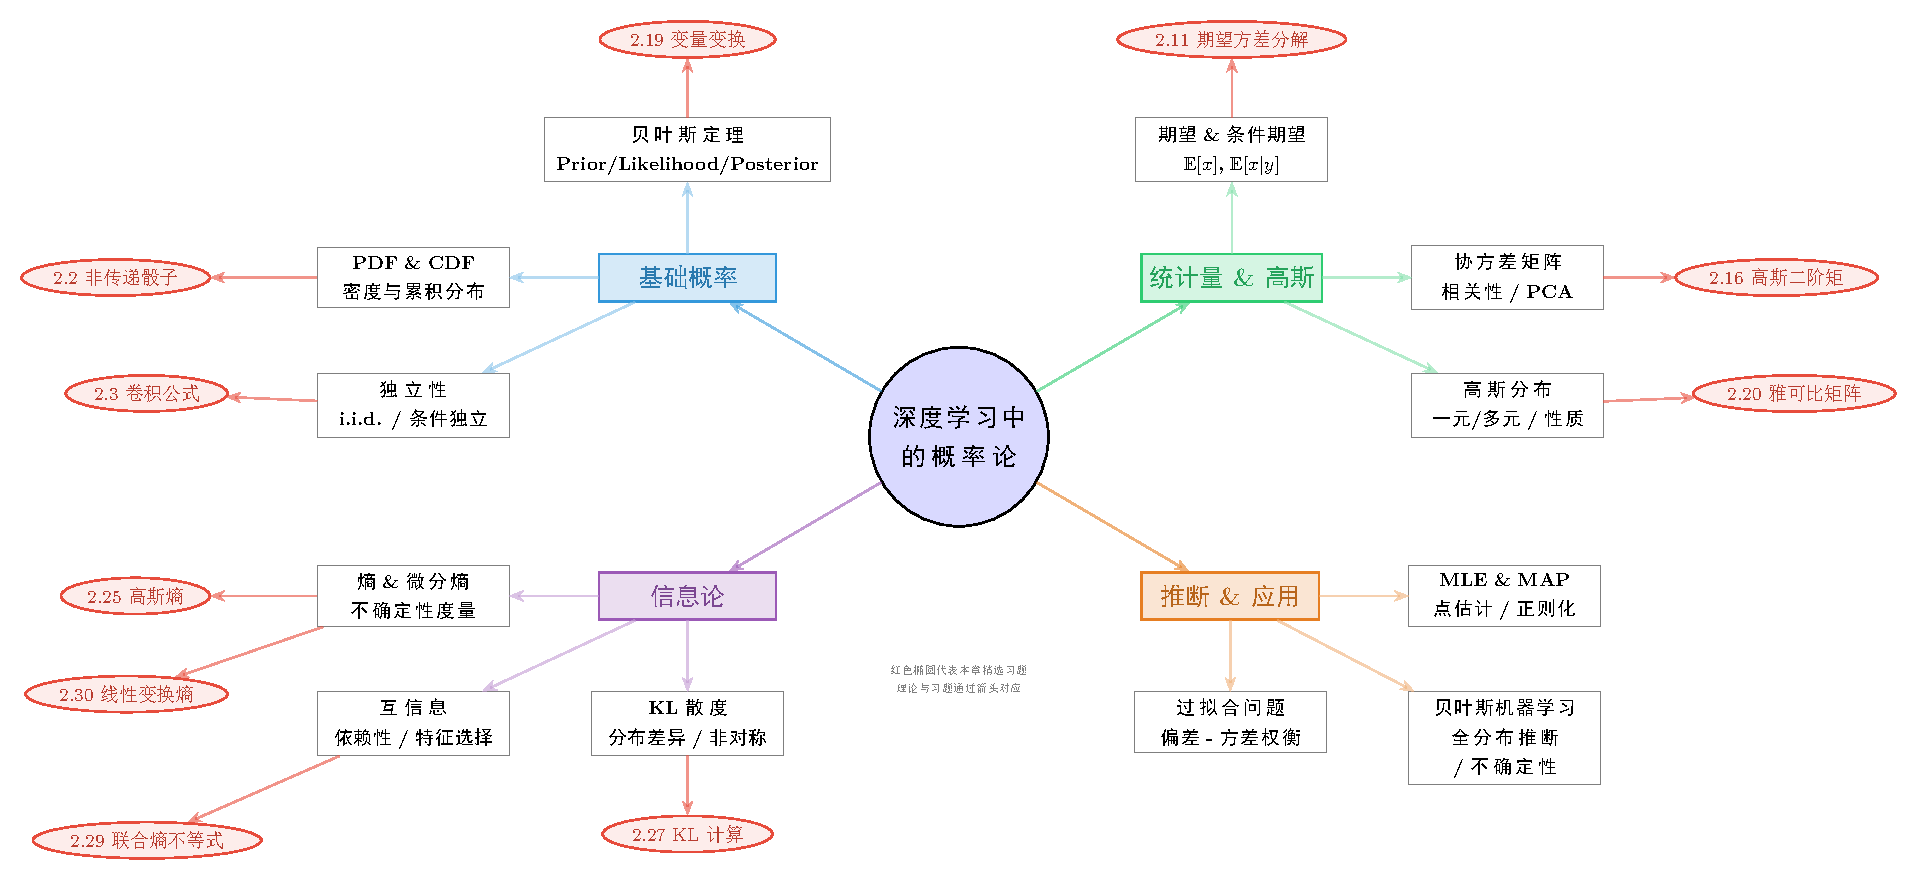
\includegraphics[width=0.95\textwidth]{ch02-graph.pdf}
    \end{center}
\end{frame}


\section{基础概率与贝叶斯定理}

% 1. Bayes' theorem
\begin{frame}{贝叶斯定理 (Bayes' Theorem)}
    \begin{itemize}
        \item \textbf{定义}：描述两个事件 $A$ 和 $B$ 之间条件概率关系的定理，是贝叶斯统计学的基石。
        \item \textbf{公式}：
        $\displaystyle P(A|B) = \frac{P(B|A) P(A)}{P(B)} $
        \item \textbf{在机器学习中的形式}：
        $\displaystyle p(\boldsymbol{\theta}|D) = \frac{p(D|\boldsymbol{\theta}) p(\boldsymbol{\theta})}{p(D)} $
        \begin{itemize}
            \item $p(\boldsymbol{\theta}|D)$：后验概率 (Posterior)。
            \item $p(D|\boldsymbol{\theta})$：似然 (Likelihood)。
            \item $p(\boldsymbol{\theta})$：先验 (Prior)。
            \item $p(D)$：证据 (Evidence) 或边缘似然。
        \end{itemize}
        \item \textbf{意义}：提供了从“数据更新信念”的数学框架。我们将先验知识结合观测数据，得到更新后的参数分布。
    \end{itemize}
\end{frame}

% 2. Prior probability
\begin{frame}{先验概率 (Prior Probability)}
    \begin{itemize}
        \item \textbf{定义}：在观测到任何数据之前，对参数 $\boldsymbol{\theta}$ 或事件 $A$ 的概率分布的初始信念。
        \item \textbf{表示}：$p(\boldsymbol{\theta})$ 或 $P(A)$。
        \item \textbf{作用}：
        \begin{itemize}
            \item 引入领域知识（例如：权重通常较小，可用高斯先验）。
            \item 起到正则化的作用，防止模型过度依赖少量数据。
        \end{itemize}
        \item \textbf{类型}：
        \begin{itemize}
            \item \textbf{信息性先验 (Informative Prior)}：基于具体知识设定（如 $\boldsymbol{\theta} \sim \N(0, 1)$）。
            \item \textbf{非信息性先验 (Non-informative Prior)}：表示无知（如均匀分布）。
        \end{itemize}
        \item \textbf{深度学习中}：L2 正则化等价于高斯先验，L1 正则化等价于拉普拉斯先验。
    \end{itemize}
\end{frame}

% 3. Posterior probability
\begin{frame}{后验概率 (Posterior Probability)}
    \begin{itemize}
        \item \textbf{定义}：在观测到数据 $D$ 之后，对参数 $\boldsymbol{\theta}$ 或类别 $C_k$ 的更新后的概率分布。
        \item \textbf{表示}：$p(\boldsymbol{\theta}|D)$ 或 $P(C_k|\vect{x})$。
        \item \textbf{核心地位}：
        \begin{itemize}
            \item 是贝叶斯推断的最终目标。
            \item 包含了数据和先验的所有信息。
        \end{itemize}
        \item \textbf{在分类中的应用}：
        \begin{itemize}
            \item 判别式模型直接建模 $p(C_k|\vect{x})$。
            \item 生成式模型通过贝叶斯定理计算 $p(C_k|\vect{x}) \propto p(\vect{x}|C_k)p(C_k)$。
        \end{itemize}
        \item \textbf{挑战}：计算分母 $p(D)$ 通常涉及高维积分，难以解析求解，需借助近似推断（MCMC, 变分推断）。
    \end{itemize}
\end{frame}

% 4. Independent variables
\begin{frame}{独立变量 (Independent Variables)}
    \begin{itemize}
        \item \textbf{定义}：两个随机变量 $X$ 和 $Y$ 如果满足 $P(X, Y) = P(X)P(Y)$，则称它们相互独立。
        \item \textbf{条件独立}：给定 $Z$ 时，$X$ 和 $Y$ 独立，记为 $X \perp Y | Z$，即 $P(X, Y|Z) = P(X|Z)P(Y|Z)$。
        \item \textbf{在深度学习中的假设}：
        \begin{itemize}
            \item \textbf{i.i.d. 假设}：训练数据样本之间通常是独立同分布 (Independent and Identically Distributed) 的。这使得似然函数可以写成连乘形式：$L = \prod p(x_i)$。
            \item \textbf{朴素贝叶斯}：假设特征之间条件独立，极大地简化了计算。
        \end{itemize}
        \item \textbf{注意}：在序列数据（如时间序列、文本）中，独立性假设通常不成立，需使用 RNN 或 Transformer 建模依赖关系。
    \end{itemize}
\end{frame}

% 5. Probability density function (PDF)
\begin{frame}{概率密度函数 (Probability Density Function, PDF)}
    \begin{itemize}
        \item \textbf{定义}：描述连续型随机变量 $x$ 在某个特定取值点附近的相对可能性。记为 $p(x)$。
        \item \textbf{性质}：
        \begin{itemize}
            \item 非负性：$p(x) \ge 0$。
            \item 归一化：$\int_{-\infty}^{\infty} p(x) dx = 1$。
            \item 概率计算：$x$ 落在区间 $[a, b]$ 的概率为 $\int_a^b p(x) dx$。
        \end{itemize}
        \item \textbf{区别}：$p(x)$ 的值本身不是概率（可以大于 1），只有积分才是概率。
        \item \textbf{应用}：定义损失函数（如负对数似然）、生成模型的目标分布。
    \end{itemize}
\end{frame}

% 6. Cumulative distribution function (CDF)
\begin{frame}{累积分布函数 (Cumulative Distribution Function, CDF)}
    \begin{itemize}
        \item \textbf{定义}：随机变量 $X$ 小于或等于某个值 $x$ 的概率。
        $$ F(x) = P(X \le x) = \int_{-\infty}^x p(t) dt $$
        \item \textbf{性质}：
        \begin{itemize}
            \item 单调不减。
            \item $F(-\infty) = 0, F(\infty) = 1$。
            \item 与 PDF 的关系：$p(x) = \frac{d}{dx} F(x)$。
        \end{itemize}
        \item \textbf{应用}：
        \begin{itemize}
            \item \textbf{逆变换采样}：若 $u \sim U[0,1]$，则 $x = F^{-1}(u)$ 服从分布 $F$。常用于生成模型采样。
            \item 计算分位数（如中位数）。
        \end{itemize}
    \end{itemize}
\end{frame}

\section{统计量与高斯分布}

% 7. Expectation
\begin{frame}{期望 (Expectation)}
    \begin{itemize}
        \item \textbf{定义}：随机变量取值的加权平均，权重为概率。
        \item \textbf{公式}：
        \begin{itemize}
            \item 离散：$\E[f(x)] = \sum_x p(x) f(x)$
            \item 连续：$\E[f(x)] = \int p(x) f(x) dx$
        \end{itemize}
        \item \textbf{线性性质}：$\E[ax + by] = a\E[x] + b\E[y]$，无论 $x, y$ 是否独立。
        \item \textbf{经验期望}：在机器学习中，通常用样本均值近似总体期望：
        $$ \E[f(x)] \approx \frac{1}{N} \sum_{n=1}^N f(x_n) $$
        \item \textbf{应用}：损失函数的定义（期望风险）、梯度下降中的期望梯度。
    \end{itemize}
\end{frame}

% 8. Covariance
\begin{frame}{协方差 (Covariance)}
    \begin{itemize}
        \item \textbf{定义}：衡量两个随机变量 $x$ 和 $y$ 之间的线性相关程度。
        $$ \text{Cov}[x, y] = \E[(x - \E[x])(y - \E[y])] = \E[xy] - \E[x]\E[y] $$
        \item \textbf{协方差矩阵}：对于随机向量 $\vect{x}$，$\boldsymbol{\Sigma} = \E[(\vect{x}-\boldsymbol{\mu})(\vect{x}-\boldsymbol{\mu})^T]$。
        \item \textbf{解释}：
        \begin{itemize}
            \item $\text{Cov} > 0$：正相关（同向变化）。
            \item $\text{Cov} < 0$：负相关（反向变化）。
            \item $\text{Cov} = 0$：不相关（但不一定独立，除非是高斯分布）。
        \end{itemize}
        \item \textbf{深度学习应用}：
        \begin{itemize}
            \item PCA（主成分分析）基于协方差矩阵的特征分解。
            \item Batch Normalization 利用批内协方差统计量进行归一化。
            \item 自注意力机制 (Self-Attention) 本质上在建模 token 间的协方差关系。
        \end{itemize}
    \end{itemize}
\end{frame}

% 9. Conditional expectation
\begin{frame}{条件期望 (Conditional Expectation)}
    \begin{itemize}
        \item \textbf{定义}：在已知随机变量 $Y=y$ 的条件下，$X$ 的期望值。记为 $\E[X|Y=y]$。
        $$ \E[X|Y] = \int x \, p(x|Y) dx $$
        \item \textbf{作为函数}：$\E[X|Y]$ 本身是一个关于 $Y$ 的随机变量。
        \item \textbf{回归的最优解}：
        \begin{itemize}
            \item 在最小化平方损失 $L = (y - t)^2$ 的意义下，最优预测函数 $y(\vect{x})$ 就是目标变量的条件期望：
            $$ y^*(\vect{x}) = \E[t|\vect{x}] $$
        \end{itemize}
        \item \textbf{全期望公式}：$\E[X] = \E[\E[X|Y]]$。
    \end{itemize}
\end{frame}

% 10. Gaussian distribution
\begin{frame}{高斯分布 (Gaussian Distribution)}
    \begin{itemize}
        \item \textbf{别名}：正态分布 (Normal Distribution)。
        \item \textbf{重要性}：由中心极限定理支撑，是深度学习和统计学中最核心的分布。
        \item \textbf{一元形式}：
        $$ \N(x|\mu, \sigma^2) = \frac{1}{\sqrt{2\pi\sigma^2}} \exp\left(-\frac{(x-\mu)^2}{2\sigma^2}\right) $$
        \item \textbf{多元形式}：
        $$ \N(\vect{x}|\boldsymbol{\mu}, \boldsymbol{\Sigma}) = \frac{1}{(2\pi)^{D/2}|\boldsymbol{\Sigma}|^{1/2}} \exp\left(-\frac{1}{2}(\vect{x}-\boldsymbol{\mu})^T\boldsymbol{\Sigma}^{-1}(\vect{x}-\boldsymbol{\mu})\right) $$
        \item \textbf{关键性质}：
        \begin{itemize}
            \item 完全由一阶矩（均值）和二阶矩（协方差）决定。
            \item 线性变换后仍为高斯。
            \item 边缘分布和条件分布仍为高斯。
        \end{itemize}
    \end{itemize}
\end{frame}

% 11. Likelihood function
\begin{frame}{似然函数 (Likelihood Function)}
    \begin{itemize}
        \item \textbf{定义}：给定数据 $D$ 下，关于参数 $\boldsymbol{\theta}$ 的函数，形式上等于联合概率密度，但视角不同。
        $$ L(\boldsymbol{\theta}) = p(D|\boldsymbol{\theta}) = \prod_{n=1}^N p(\vect{x}_n|\boldsymbol{\theta}) $$
        \item \textbf{与概率的区别}：
        \begin{itemize}
            \item 概率：固定参数，预测数据。
            \item 似然：固定数据，评估参数。
        \end{itemize}
        \item \textbf{最大似然估计 (MLE)}：寻找 $\boldsymbol{\theta}_{ML}$ 使得 $L(\boldsymbol{\theta})$ 最大。
        \item \textbf{对数似然}：为了方便计算，通常最大化 $\ln L(\boldsymbol{\theta})$，将连乘转为求和。
        \item \textbf{联系}：最小化平方和误差等价于在高斯噪声假设下的最大似然估计。
    \end{itemize}
\end{frame}

\section{信息论基础}

% 12. Entropy of the random variable
\begin{frame}{随机变量的熵 (Entropy)}
    \begin{itemize}
        \item \textbf{定义}：衡量随机变量不确定性的度量，或编码该变量所需的最小平均比特数。
        $$ \mcH[x] = -\sum_x p(x) \log_2 p(x) \quad (\text{离散}) $$
        $$ \mcH[x] = -\int p(x) \ln p(x) dx \quad (\text{连续，即微分熵}) $$
        \item \textbf{性质}：
        \begin{itemize}
            \item 熵越大，不确定性越高，分布越均匀。
            \item 熵越小，确定性越高，分布越集中。
            \item 对于离散变量，均匀分布时熵最大。
        \end{itemize}
        \item \textbf{应用}：
        \begin{itemize}
            \item 决策树分裂标准（信息增益）。
            \item 强化学习中的最大熵探索。
            \item 生成模型的目标（最大化生成数据的似然等价于最小化交叉熵）。
        \end{itemize}
    \end{itemize}
\end{frame}

% 13. Differential entropy
\begin{frame}{微分熵 (Differential Entropy)}
    \begin{itemize}
        \item \textbf{定义}：连续随机变量的熵。
        $$ \mcH[x] = -\int p(x) \ln p(x) dx $$
        \item \textbf{与离散熵的区别}：
        \begin{itemize}
            \item 可以为负值（因为概率密度 $p(x)$ 可以大于 1）。
            \item 不具有坐标变换不变性（随变量缩放而变化）。
            \item 不代表绝对的最小编码长度，而是相对于均匀分布的相对度量。
        \end{itemize}
        \item \textbf{高斯分布的微分熵}：
        $$ \mcH[\N(\mu, \sigma^2)] = \frac{1}{2} \ln(2\pi e \sigma^2) $$
        在所有具有相同方差的分布中，高斯分布的微分熵最大。
    \end{itemize}
\end{frame}

% 14. Relative entropy / KL divergence
\begin{frame}{相对熵 / KL 散度 (Relative Entropy / KL Divergence)}
    \begin{itemize}
        \item \textbf{定义}：衡量两个概率分布 $p(x)$ 和 $q(x)$ 之间的差异（非对称距离）。
        $$ \KL(p||q) = -\int p(x) \ln \frac{q(x)}{p(x)} dx = \E_{p(x)}[\ln p(x)] - \E_{p(x)}[\ln q(x)] $$
        \item \textbf{性质}：
        \begin{itemize}
            \item 非负性：$\KL(p||q) \ge 0$，当且仅当 $p=q$ 时取等号。
            \item 非对称性：$\KL(p||q) \neq \KL(q||p)$。
        \end{itemize}
        \item \textbf{深度学习应用}：
        \begin{itemize}
            \item \textbf{变分自编码器 (VAE)}：损失函数包含 KL 散度项，用于约束潜变量分布接近先验（通常是标准高斯）。
            \item \textbf{强化学习}：约束策略更新幅度 (PPO, TRPO)。
            \item \textbf{蒸馏}：让学生网络的输出分布逼近教师网络。
        \end{itemize}
    \end{itemize}
\end{frame}

% 15. Conditional entropy
\begin{frame}{条件熵 (Conditional Entropy)}
    \begin{itemize}
        \item \textbf{定义}：在已知随机变量 $Y$ 的条件下，$X$ 的不确定性。
        $$ \mcH[X|Y] = \sum_y p(y) \mcH[X|Y=y] = -\sum_{x,y} p(x,y) \ln p(x|y) $$
        \item \textbf{链式法则}：
        $$ \mcH[X, Y] = \mcH[Y] + \mcH[X|Y] $$
        联合熵等于 $Y$ 的熵加上已知 $Y$ 后 $X$ 的剩余熵。
        \item \textbf{性质}：$\mcH[X|Y] \le \mcH[X]$。知道更多信息（$Y$）只会减少或保持不确定性，不会增加。
        \item \textbf{应用}：定义互信息的基础。
    \end{itemize}
\end{frame}

% 16. Mutual information
\begin{frame}{互信息 (Mutual Information)}
    \begin{itemize}
        \item \textbf{定义}：衡量两个随机变量 $X$ 和 $Y$ 之间相互依赖程度的量。
        $$ I[X; Y] = \mcH[X] - \mcH[X|Y] = \mcH[Y] - \mcH[Y|X] $$
        也可以表示为联合分布与边缘分布乘积的 KL 散度：
        $$ I[X; Y] = \KL(p(x,y) || p(x)p(y)) $$
        \item \textbf{解释}：知道 $Y$ 后，$X$ 的不确定性减少了多少。
        \item \textbf{性质}：
        \begin{itemize}
            \item 对称性：$I[X; Y] = I[Y; X]$。
            \item 非负性：$I[X; Y] \ge 0$。
            \item 若独立，则 $I[X; Y] = 0$。
        \end{itemize}
        \item \textbf{应用}：
        \begin{itemize}
            \item 特征选择。
            \item InfoGAN：最大化潜变量与生成图像部分的互信息以解耦特征。
            \item Deep InfoMax：最大化局部与全局特征的互信息进行无监督学习。
        \end{itemize}
    \end{itemize}
\end{frame}

\section{推断与机器学习应用}

% 17. Problem of over-fitting
\begin{frame}{过拟合问题 (Problem of Over-fitting)}
    \begin{itemize}
        \item \textbf{定义}：模型在训练数据上表现极好（误差低），但在未见过的测试数据上表现差（泛化能力弱）。
        \item \textbf{原因}：
        \begin{itemize}
            \item 模型过于复杂（参数过多），记住了训练数据的噪声而非规律。
            \item 训练数据量不足。
        \end{itemize}
        \item \textbf{概率视角}：
        \begin{itemize}
            \item 最大似然估计 (MLE) 倾向于选择极其复杂的模型以完美拟合数据，导致过拟合。
            \item MLE 没有考虑参数的先验信念。
        \end{itemize}
        \item \textbf{解决方案}：
        \begin{itemize}
            \item 正则化 (Regularization)。
            \item 贝叶斯方法 (引入先验)。
            \item Dropout, 数据增强，早停法 (Early Stopping)。
        \end{itemize}
    \end{itemize}
\end{frame}

% 18. Sum-of-squares error function
\begin{frame}{平方和误差函数 (Sum-of-Squares Error Function)}
    \begin{itemize}
        \item \textbf{定义}：最常用的回归损失函数。
        $$ E(\vect{w}) = \frac{1}{2} \sum_{n=1}^N (y(\vect{x}_n, \vect{w}) - t_n)^2 $$
        \item \textbf{概率推导}：
        \begin{itemize}
            \item 假设目标值 $t$ 由模型输出加高斯噪声生成：$t = y(\vect{x}, \vect{w}) + \epsilon, \quad \epsilon \sim \N(0, \beta^{-1})$。
            \item 此时，最大化似然函数 $\ln p(D|\vect{w})$ 等价于最小化平方和误差。
        \end{itemize}
        \item \textbf{缺点}：对异常值（Outliers）敏感，因为误差被平方放大。
        \item \textbf{扩展}：加入正则化项 $\frac{\lambda}{2}\|\vect{w}\|^2$ 即为正则化最小二乘法。
    \end{itemize}
\end{frame}

% 19. Maximum a posteriori estimate (MAP)
\begin{frame}{最大后验估计 (Maximum A Posteriori Estimate, MAP)}
    \begin{itemize}
        \item \textbf{定义}：寻找使后验概率 $p(\boldsymbol{\theta}|D)$ 最大的参数值 $\boldsymbol{\theta}_{MAP}$。
        $$ \boldsymbol{\theta}_{MAP} = \arg\max_{\boldsymbol{\theta}} p(\boldsymbol{\theta}|D) = \arg\max_{\boldsymbol{\theta}} [ \ln p(D|\boldsymbol{\theta}) + \ln p(\boldsymbol{\theta}) ] $$
        \item \textbf{对比 MLE}：
        \begin{itemize}
            \item MLE: $\arg\max \ln p(D|\boldsymbol{\theta})$ (仅看数据)。
            \item MAP: $\arg\max (\ln p(D|\boldsymbol{\theta}) + \ln p(\boldsymbol{\theta}))$ (数据 + 先验)。
        \end{itemize}
        \item \textbf{正则化解释}：
        \begin{itemize}
            \item 高斯先验 $\to$ L2 正则化。
            \item 拉普拉斯先验 $\to$ L1 正则化。
        \end{itemize}
        \item \textbf{局限}：MAP 只是一个点估计，忽略了后验分布的形状（不确定性），不如全贝叶斯推断完整。
    \end{itemize}
\end{frame}

% 20. Bayesian machine learning
\begin{frame}{贝叶斯机器学习 (Bayesian Machine Learning)}
    \begin{itemize}
        \item \textbf{核心理念}：不寻求单一的“最佳”参数点，而是计算参数的完整后验分布 $p(\boldsymbol{\theta}|D)$。
        \item \textbf{预测}：通过积分（边缘化）所有可能的参数进行预测：
        $$ p(t|\vect{x}, D) = \int p(t|\vect{x}, \boldsymbol{\theta}) p(\boldsymbol{\theta}|D) d\boldsymbol{\theta} $$
        \item \textbf{优势}：(1) \textbf{自然防止过拟合}：通过先验和边缘化自动实现奥卡姆剃刀原理。\\
        (2)\textbf{不确定性量化}：预测结果不仅包含值，还包含置信度（方差）。这对安全关键应用（如自动驾驶、医疗）至关重要。
        \item \textbf{挑战与方法}：
        积分通常难以计算。
        常用近似方法：变分推断 (Variational Inference, VI)、马尔可夫链蒙特卡洛 (MCMC)、拉普拉斯近似。
        \item \textbf{现代应用}：贝叶斯神经网络 (BNN)、高斯过程 (GP)、扩散模型 (Diffusion Models)。
    \end{itemize}
\end{frame}

% 结束页
\begin{frame}{总结}
    \begin{itemize}
        \item \textbf{基础}：贝叶斯定理连接了先验、似然和后验，是理解模型更新的钥匙。
        \item \textbf{统计量}：期望、协方差和高斯分布构成了建模数据分布的语言。
        \item \textbf{信息论}：熵、KL 散度和互信息提供了衡量不确定性、分布差异和信息量的工具，是许多损失函数的理论基础。
        \item \textbf{推断}：从 MLE 到 MAP 再到全贝叶斯推断，我们逐渐从点估计走向分布估计，从而更好地解决过拟合问题并量化不确定性。
        \item 掌握这些概率理论概念，是深入理解现代深度学习算法（如 VAE, GAN, Transformer, Diffusion）的前提。
    \end{itemize}
\end{frame}

\end{document}
